\documentclass{beamer}
% \usepackage[utf8]{inputenc}
\usepackage[T1]{fontenc}
\usetheme{CambridgeUS}
\useoutertheme{miniframes}
\usecolortheme{dove}
\usefonttheme{serif}
\beamertemplatenavigationsymbolsempty

\usepackage[english]{babel}
% \usepackage[english, polish]{babel}

\usepackage{listings}
\lstset{basicstyle=\ttfamily\footnotesize,breaklines=true}
\usepackage{siunitx}
\usepackage{mhchem}
\usepackage{pifont}
\usepackage{amsmath,amssymb,amsfonts}
\usepackage{graphicx}
\usepackage[export]{adjustbox}
\usepackage{float}
\usepackage{xcolor}
\usepackage{setspace}

\newcommand{\todo}[1]{\textcolor{red}{TODO: #1}}

\newcommand{\imagesource}[1]{
    \begin{spacing}{0.5}
        \texttt{\textit{ \tiny{source: #1}}}
    \end{spacing}
}

\newenvironment{columnframe}[1]{
    \begin{frame}[environment=columnframe,fragile]{#1}
        \begin{columns}
            }{
        \end{columns}
    \end{frame}
}


\title{Enhanced Radars}
    \subtitle{Electromagnetic Properties of Rydberg Atoms}
\author{Tobiasz Fic}
\date{28 May 2024}

\begin{document}

\begin{frame}
    \maketitle
    \begin{figure}
        \centering
        
\includegraphics[width=0.6\textwidth]{images/logo_eng.png}
    \end{figure}
\end{frame}

\begin{columnframe}{RADAR 101}
    \begin{column}{0.5\textwidth}
        \begin{figure}
            \centering
            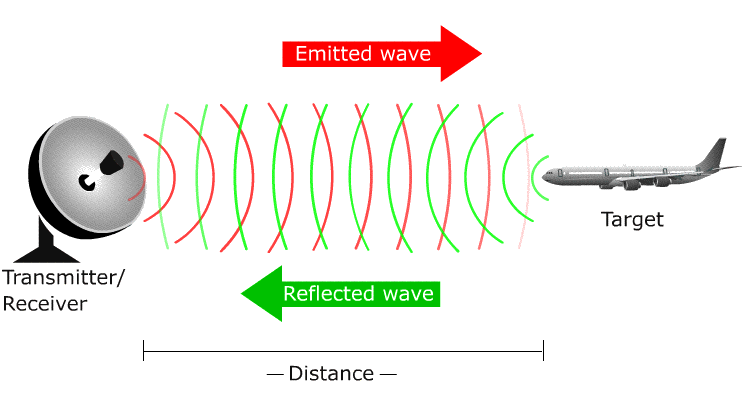
\includegraphics[width=\textwidth]{images/radar_demo.png}
            \imagesource{https://www.skyradar.com/blog/radar-principle}
        \end{figure}
    \end{column}
    \begin{column}{0.5\textwidth}
        \begin{itemize}
            \item In one sentence: send an RF signal, measure the time it takes to return, then calculate the distance.
            \item Precision is heavily dependent on our ability to measure sub-quantities.
        \end{itemize}
    \end{column}
\end{columnframe}

\begin{columnframe}{What can we use radars for?}
    \begin{column}{0.5\textwidth}
        \begin{itemize}
            \item Originally: military applications
            \item Nowadays: weather forecasting, air traffic control, speed cameras, land surveying, etc.
        \end{itemize}
    \end{column}
    \begin{column}{0.5\textwidth}
        \begin{figure}
            \centering
            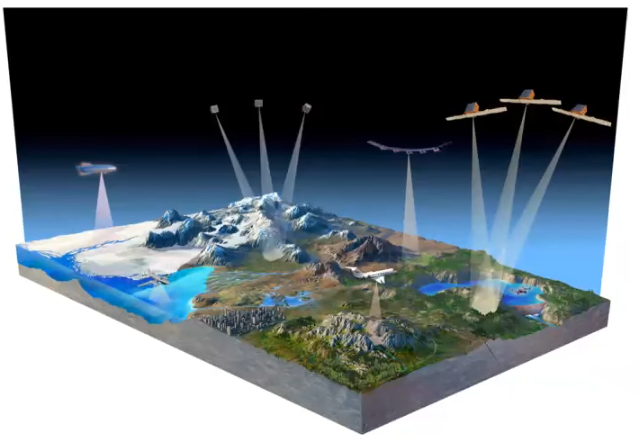
\includegraphics[width=\textwidth]{images/satellite_demo.png}
            \imagesource{Darmindra Arumugam (NASA): Quantum Rydberg Radar (presentation)}
        \end{figure}
    \end{column}
\end{columnframe}



\begin{columnframe}{Conventional RF sensing}
    \begin{column}{0.5\textwidth}
        \begin{figure}
            \centering
            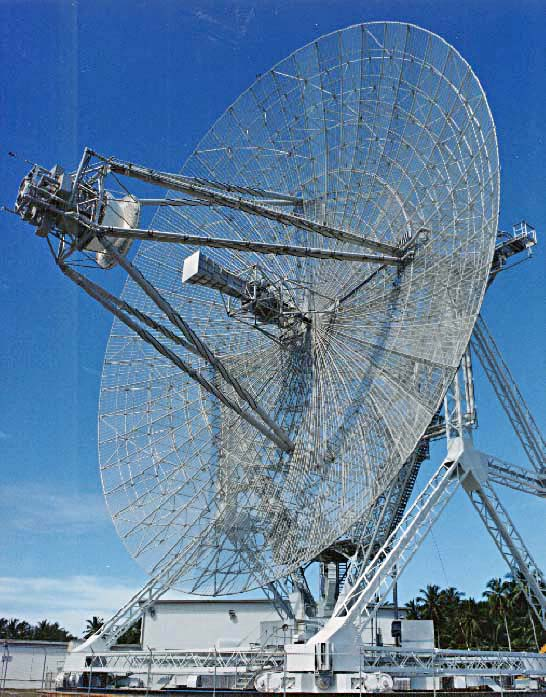
\includegraphics[width=0.8\textwidth]{images/radar_antenna_huge.jpg}
            \imagesource{https://en.wikipedia.org/wiki/Radar}
        \end{figure}
    \end{column}
    \begin{column}{0.5\textwidth}
        \begin{itemize}
            \item The simplest RF sensor is a dipole antenna - turning electric field disturbances into voltage
            \item Notoriously difficult to calibrate
            \item Made of metal, so they interfere with the signal
            \item Size is dependent on the frequency (some are huge!)
        \end{itemize}
    \end{column}
\end{columnframe}

\begin{columnframe}{Rydberg atoms}
    \begin{column}{0.5\textwidth}
        \begin{itemize}
            \item A Rydberg atom is an atom in which the outer electron is in a highly excited state (high quantum number $n$).
            \item Very sensitive to disturbances in the electric field.
                  % \item Tuned with lasers, read-out with lasers
                  % \item Alkali: $Cs^{55}$, or $Rb^{37}$
        \end{itemize}
        Electron binding energy is given with the formula:
        \[
            E_B = -\dfrac{Ry}{(n - \delta_l)^2} \; : \; Ry = 13.6 \si{\electronvolt}
        \]
        $\delta_l$ - quantum defect
    \end{column}
    \begin{column}{0.5\textwidth}
        \begin{figure}
            \centering
            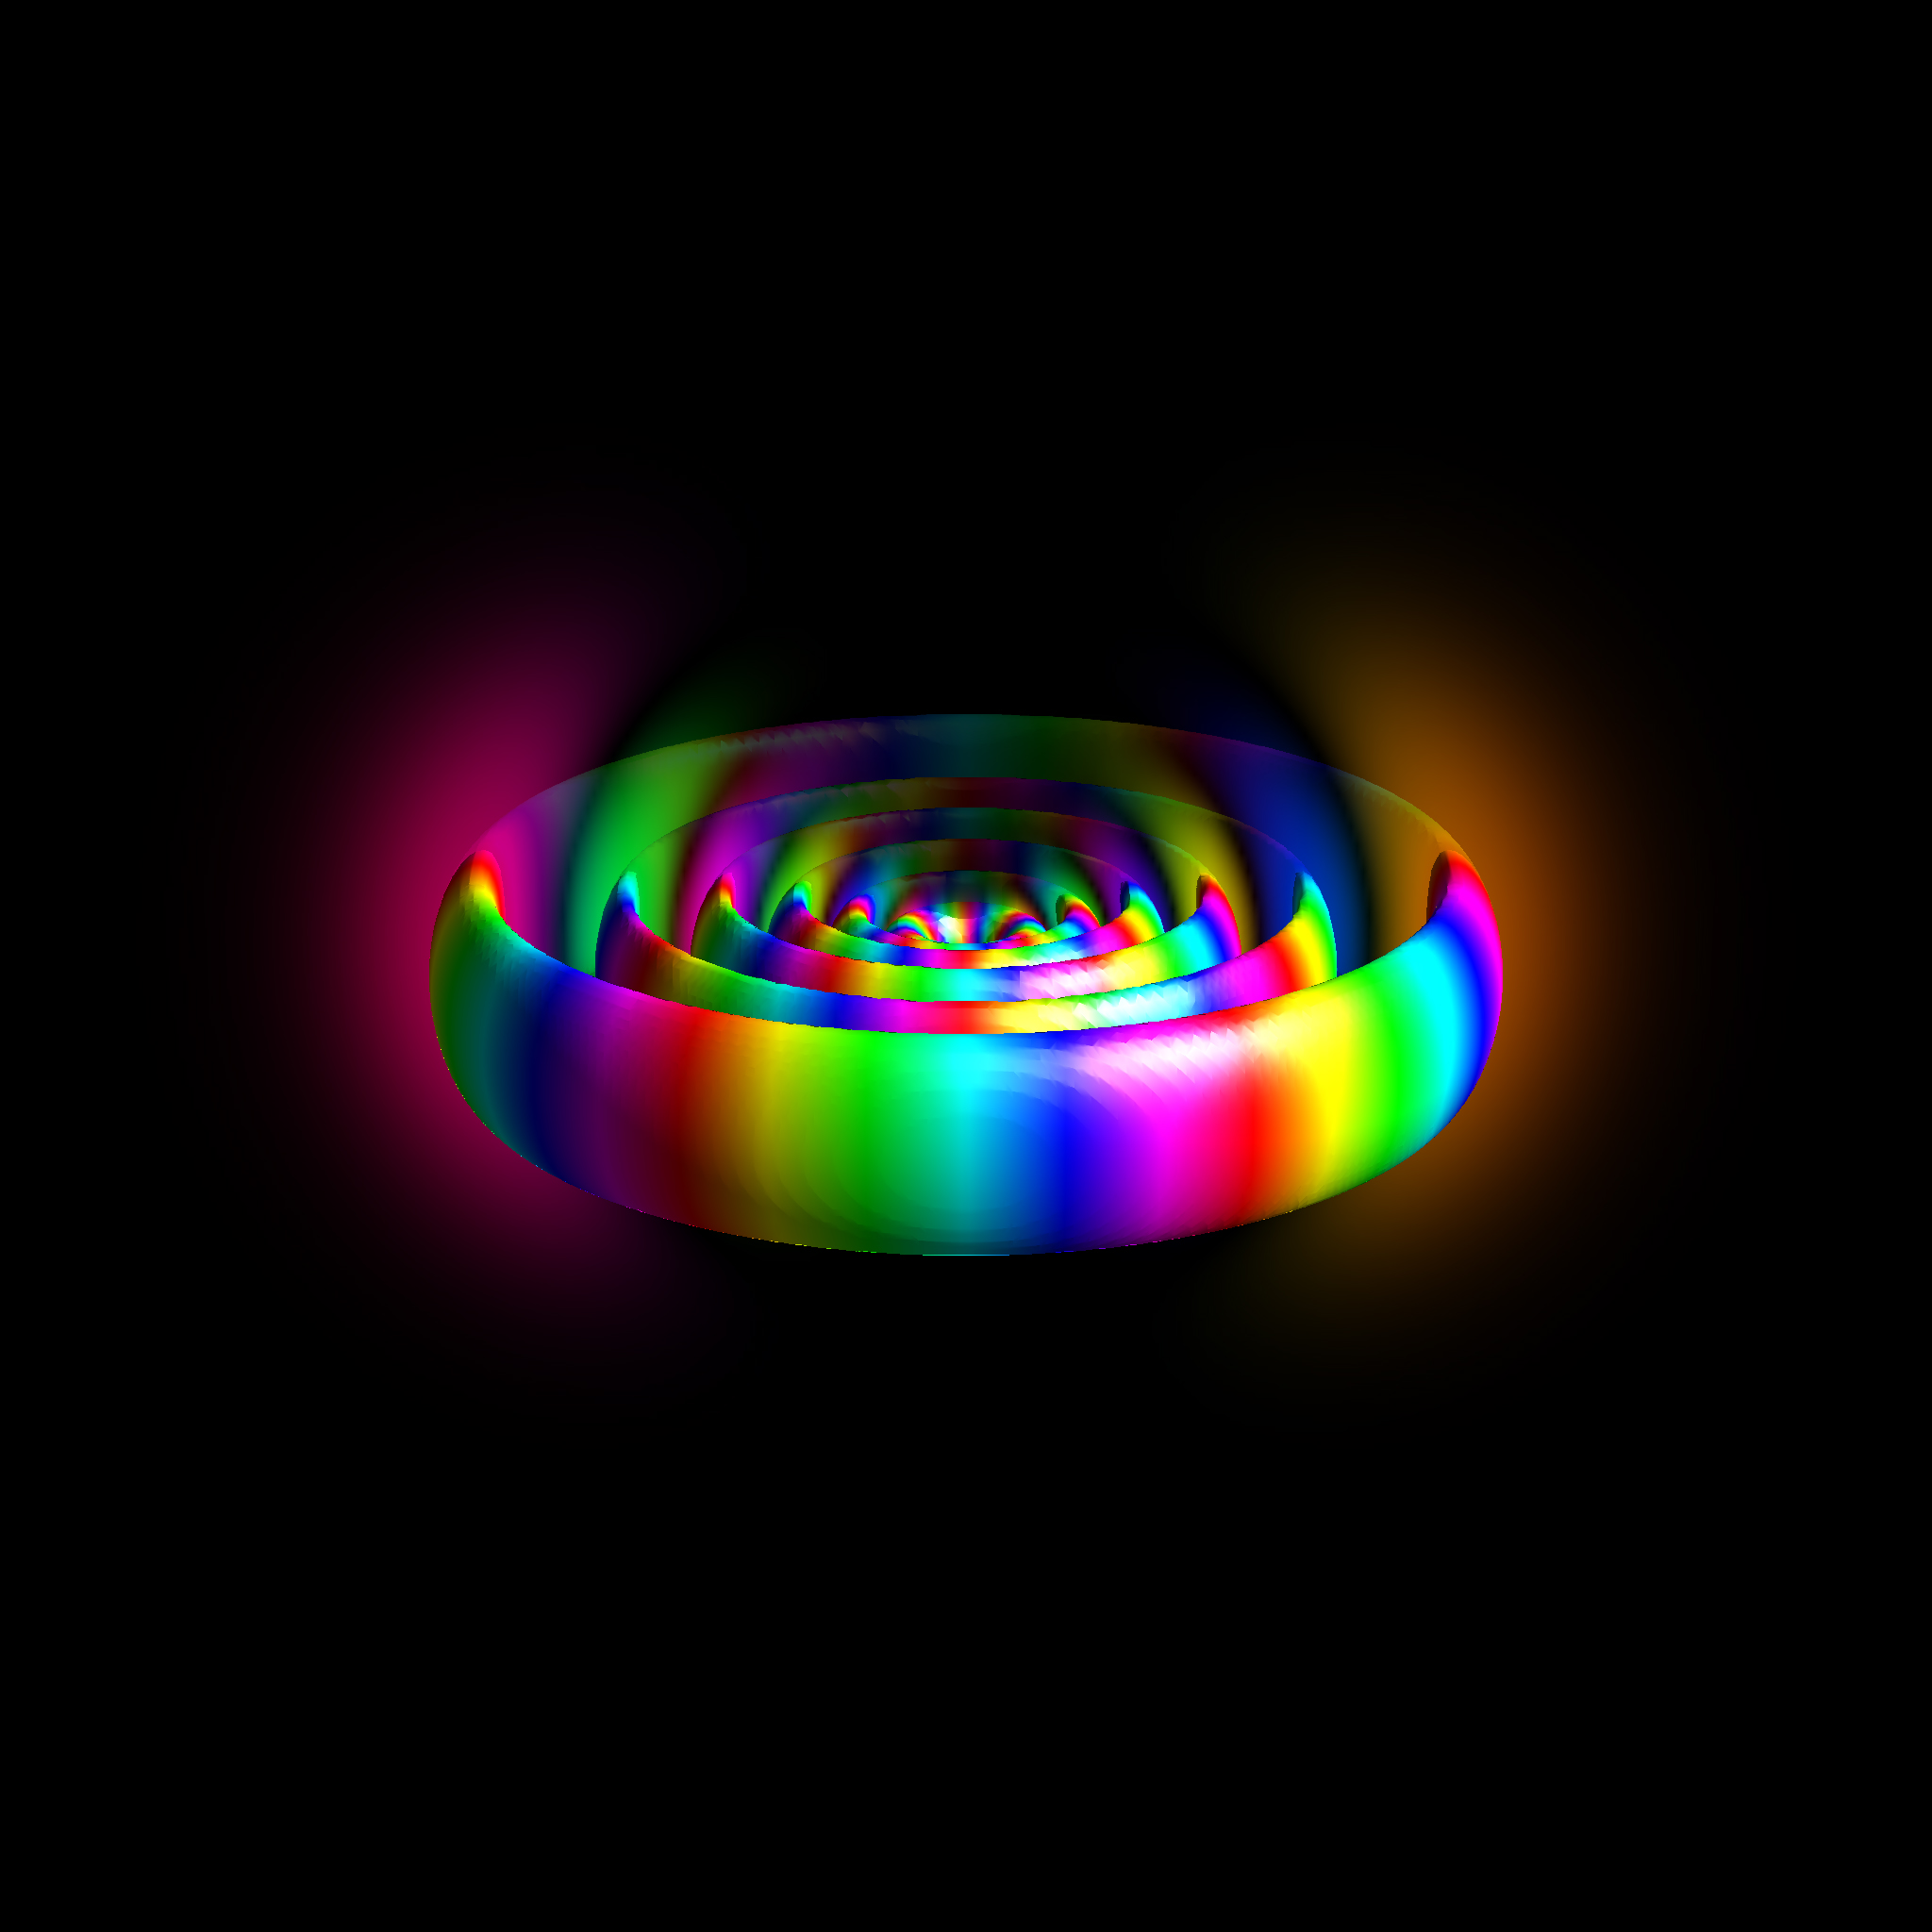
\includegraphics[width=0.7\textwidth, frame]{images/rydberg_atom_colorful.jpg}
            \caption{Orbits of a Rydberg atom with n=12, colors signify phase of the electron}
            \imagesource{https://en.wikipedia.org/wiki/Rydberg\_atom}
        \end{figure}
    \end{column}
\end{columnframe}

\begin{columnframe}{Curious properties of Alkali Metals}
    \begin{column}{0.5\textwidth}
        \begin{figure}
            \centering
            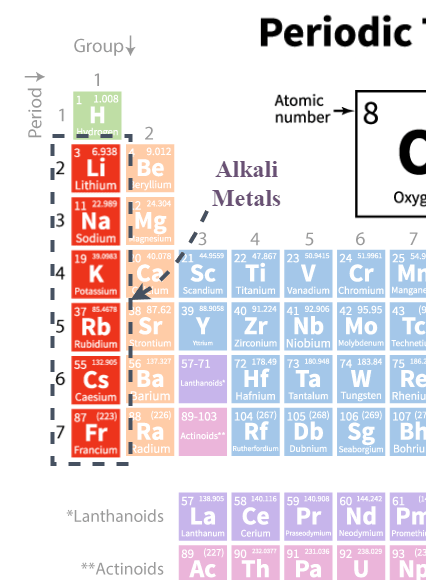
\includegraphics[width=0.7\textwidth]{images/alkali_metals_tb_of_elements.png}
            \imagesource{https://www.geeksforgeeks.org/alkali-metals/}
        \end{figure}
    \end{column}
    \begin{column}{0.5\textwidth}
        \begin{itemize}
            \item Alkali metals only have one electron on the outermost shell
            \item Easy to excite - with lasers
            \item Predictable - stable isotopes, well-studied, only the outer electron remains mobile
            \item Most commonly used: \ce{^{133}_{55}Cs}, or \ce{^{85}_{37}Rb}
        \end{itemize}
    \end{column}
\end{columnframe}

\begin{columnframe}{Detecting RF radiation with Rydberg atoms}
    \begin{column}{0.5\textwidth}
        \begin{itemize}
            \item Rydberg atoms are very sensitive to electric fields
            \item Gas - no metal - no interference
            \item Stable quantum objects
            \item Large frequency range, no size change (tuned with lasers)
            \item Scalable/portable
        \end{itemize}
    \end{column}
    \begin{column}{0.5\textwidth}
        \begin{figure}
            \centering
            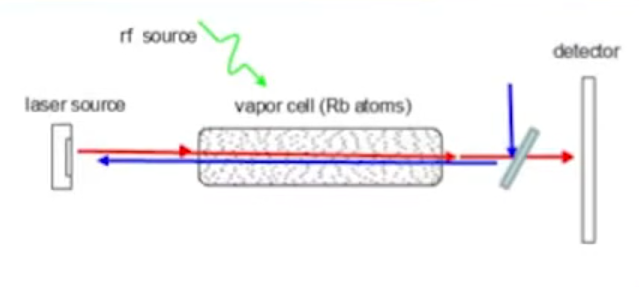
\includegraphics[width=0.8\textwidth]{images/detection_diagram.png}
            \imagesource{Chris Holloway: Rydberg Atom Based Sensors (presentation at UTC College)}
        \end{figure}
    \end{column}
\end{columnframe}

\begin{columnframe}{Measuring RF field intensity}
    \begin{column}{0.5\textwidth}
        \begin{figure}
            \centering
            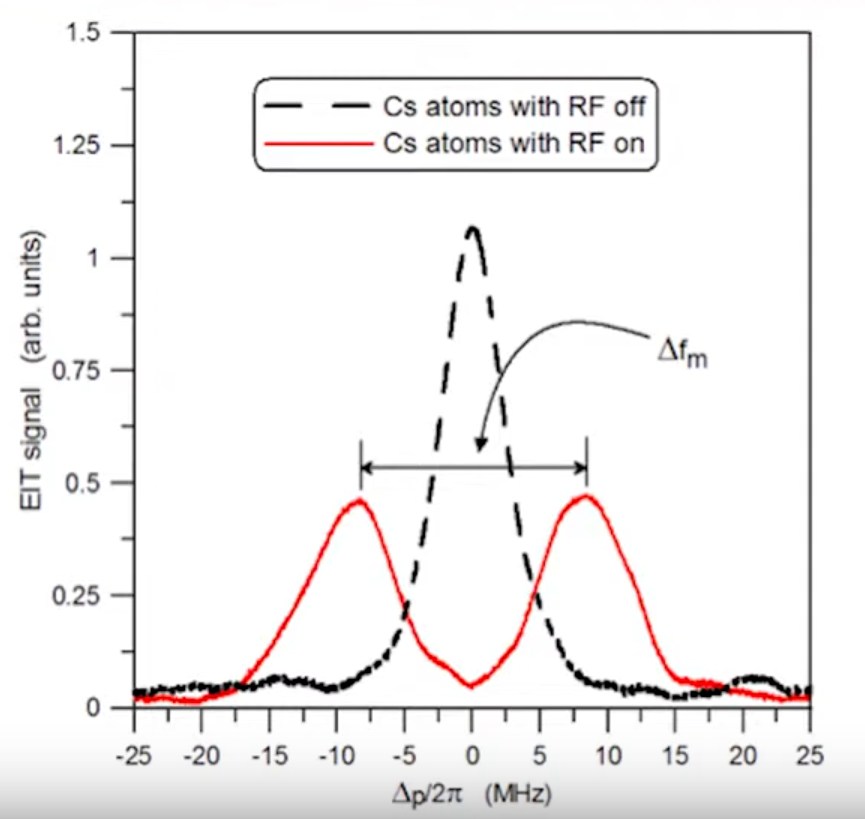
\includegraphics[width=\textwidth]{images/rydberg_eit.png}
            \imagesource{Chris Holloway: Rydberg Atom Based Sensors (presentation at UTC College)}
        \end{figure}
    \end{column}
    \begin{column}{0.5\textwidth}
        \begin{itemize}
            \item A laser is directed at the atoms to excite them
            \item A second laser is directed the other way towards a detector to read out the results via
                  Electromagnetically-Induced transparency (EIT)
            \item Distance between peaks in frequency space corresponds to intensity of field of the tuned frequency
        \end{itemize}
    \end{column}
\end{columnframe}

\begin{frame}{Measuring RF field phase}
    \begin{figure}
        \centering
        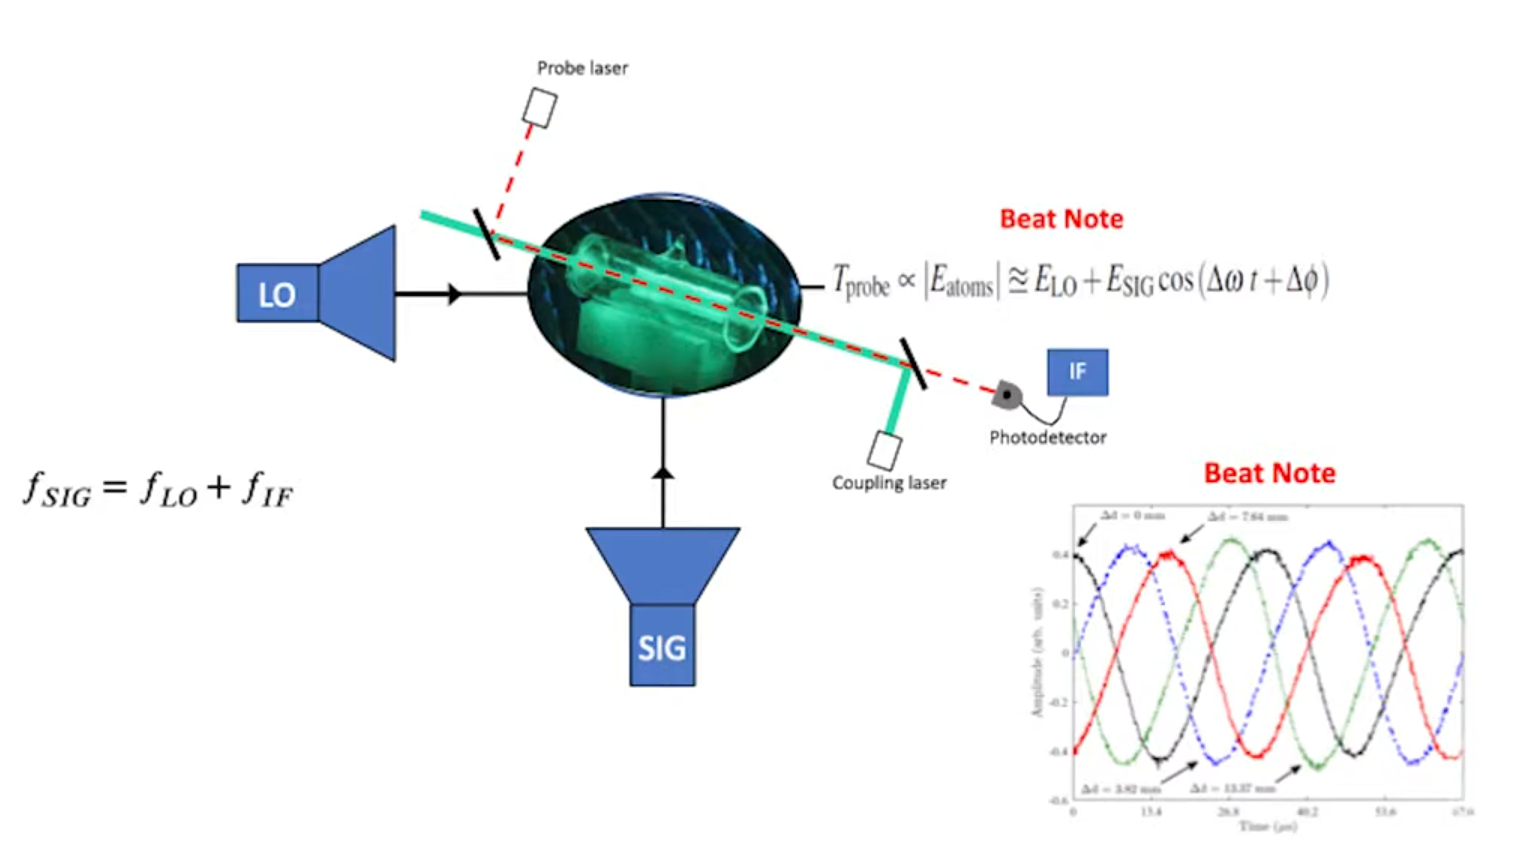
\includegraphics[width=0.8\textwidth]{images/rydberg_phase_measurement.png}
        \imagesource{Chris Holloway: Rydberg Atom Based Sensors (presentation at UTC College)}
    \end{figure}
\end{frame}

\begin{columnframe}{Repercussions}
    \begin{column}{0.9\textwidth}
        \begin{itemize}
            \item These new detectors can measure wide frequency spectrums (up to terahertz!)
            \item They are self-calibrating - properties are linked to fundamental constants
            \item They do not need to change in size relative to the frequency of interest
            \item Applications in Astronomy (RF telescope from space)
            \item Since phase measurement is possible, we can also use them for telecommunications
        \end{itemize}
    \end{column}
\end{columnframe}

\begin{columnframe}{Measuring standards}
    \begin{column}{0.48\textwidth}
        \begin{itemize}
            \item BIPM: Bureau International des Poids et Mesures (France)
            \item NIST: National Institute of Standards and Technology (USA)
            \item There is a movement to redefine SI units based on fundamental physical constants ($c$, $h$, $e$, et cetera)
            \item Electric field standards based only on Planck's constant
            \item Simplifies calibration
        \end{itemize}
    \end{column}
    \begin{column}{0.48\textwidth}
        \begin{figure}
            \centering
            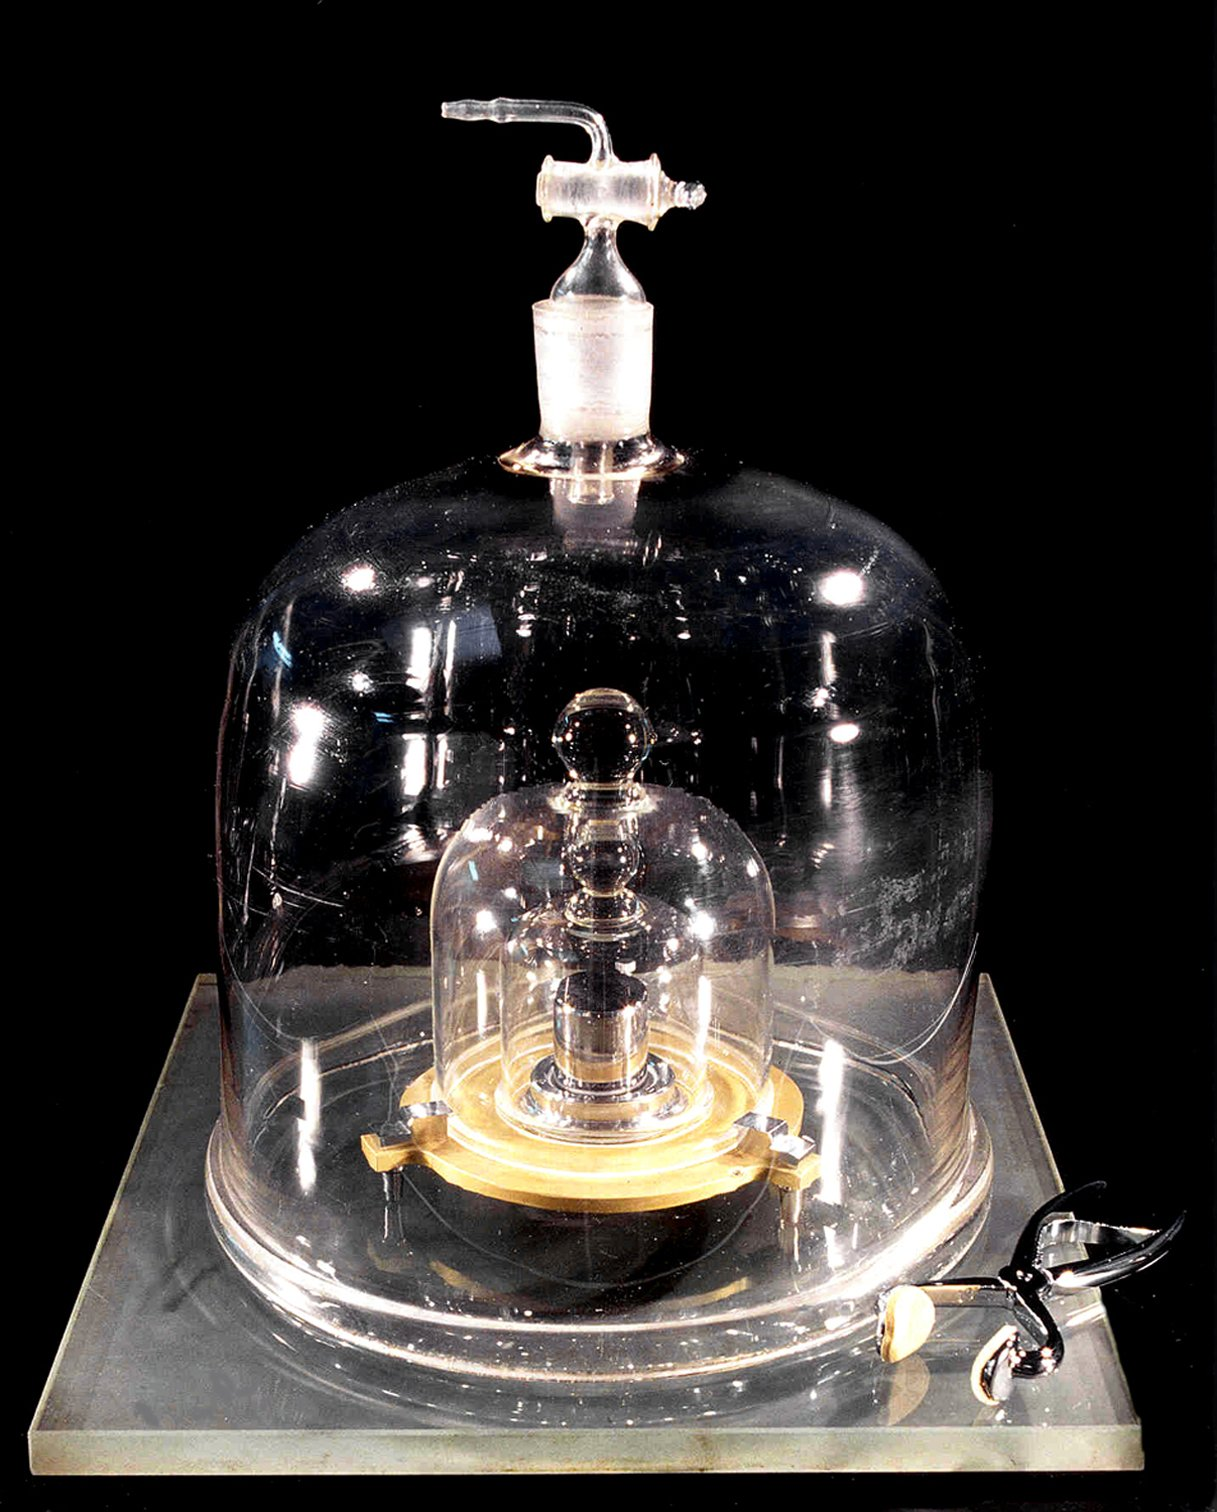
\includegraphics[width=0.8\textwidth]{images/international_prototype_of_the_kilogram.jpg}
            \imagesource{https://www.nist.gov/si-redefinition/
                kilogram-introduction}
        \end{figure}
    \end{column}
\end{columnframe}

\begin{columnframe}{Summary / Tying back to radar}
    \begin{column}{0.5\textwidth}
        \begin{figure}
            \centering
            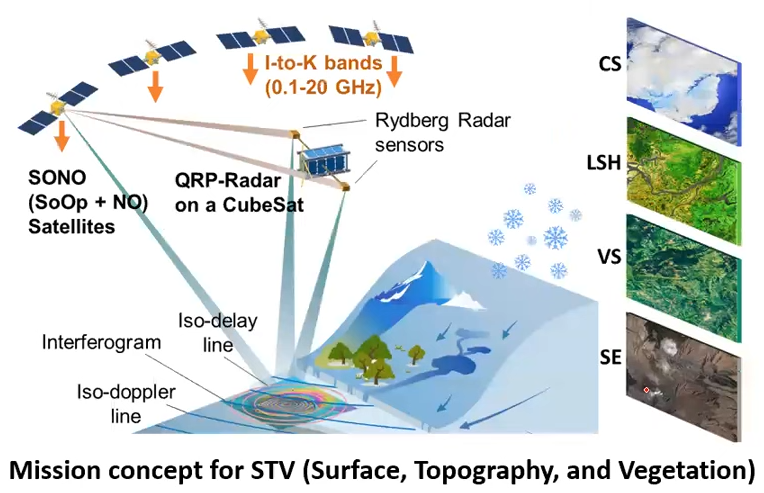
\includegraphics[width=0.8\textwidth]{images/rydberg_radar_nasa.png}
            \imagesource{Darmindra Arumugam (NASA): Quantum Rydberg Radar (presentation)}
        \end{figure}
    \end{column}
    \begin{column}{0.5\textwidth}
        \begin{itemize}
            \item Rydberg sensors would allow for a wide range of frequencies to be used in Radar
            \item They would be smaller and more accurate
            \item Feasibility has been proven, but the technology is still in its infancy
        \end{itemize}
    \end{column}
\end{columnframe}

\begin{frame}{}
    \centering
    \Large{Questions?}
\end{frame}

\begin{frame}{}
    \centering
    \Large{Thank you for your attention}
\end{frame}

\begin{frame}{Backup: phase encoding}
    \begin{figure}
        \centering
        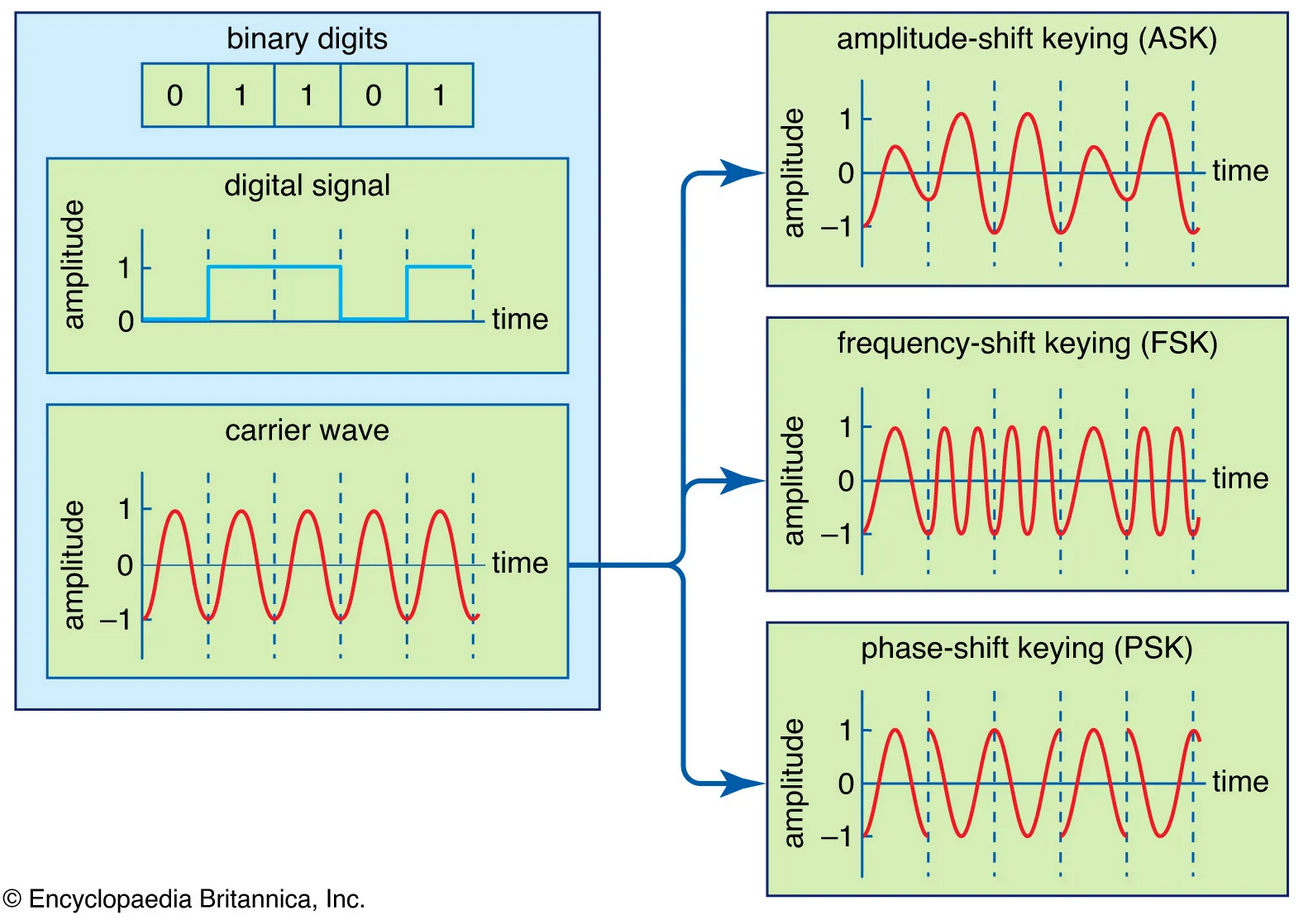
\includegraphics[width=0.8\textwidth]{images/britanicca_phase_encoding.png}
        \imagesource{Encyclopedia Britannica}
    \end{figure}
\end{frame}

\end{document}